\chapter{Experiments and Results}

\par Every collaborative task previously described was successfully implemented, but in order to validate its quality, performance, and accuracy, a series of experiments were created. They consist on quantitative and qualitative metrics and serve as a benchmark of the techniques and tasks developed in this Dissertation.

\section{Collaborative Setup}

\par The experimental setup consists on a \ac{ur10e}, with a Weiss Robotics CRG 200 gripper attachment. The vision sensor is a Microsoft Kinect \acs{rgbd} camera and the shared workspace is a simple table, approximately 50cm distant from the robot. The camera is positioned at 2m of height with a \ang{45} downwards orientation and its \ac{fov} is shown in \autoref{fig:kinect}. The complete composition of the setup is shown in \autoref{fig:setup}.

\begin{figure}[h]
    \centering
    \begin{subfigure}{.5\textwidth}
      \centering
      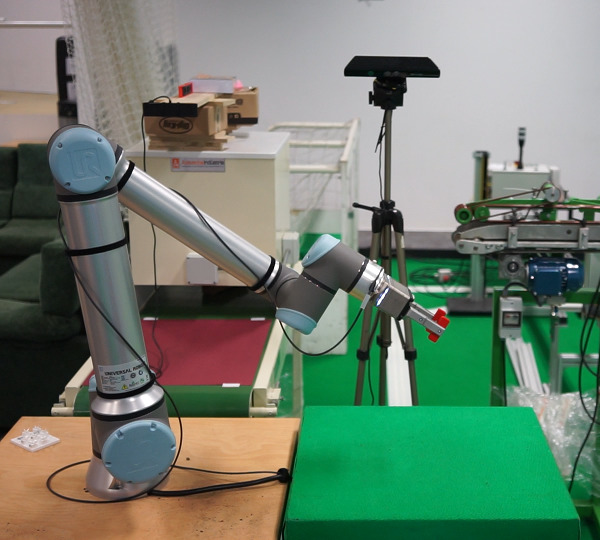
\includegraphics[width=.9\linewidth]{figs/chp6/setup.jpg}
      \caption{Collaborative Setup}
      \label{fig:setup}
    \end{subfigure}%
    \begin{subfigure}{.5\textwidth}
      \centering
      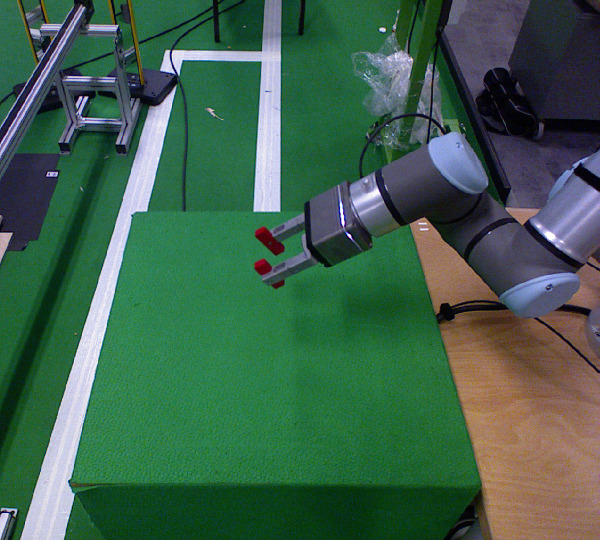
\includegraphics[width=.9\linewidth]{figs/chp6/kinect.jpg}
      \caption{Kinect \ac{fov}}
      \label{fig:kinect}
    \end{subfigure}
    \caption{Views of the experimental shared workspace}
    \label{fig:setup_and_kinect}
    \end{figure}

\section{Collaborative Tasks}

\subsection{Interaction Test}

\par To validate the use of the \ac{eef} double tap as an interaction interface with the cobot, a test case was developed in which the user would make consecutive double taps in all the directions available and observe if they were correctly registered through the colors of the gripper \acsp{led}. Each direction corresponds to a different color. A double tap interaction is considered a fail when the color of the \acsp{led} does not change, or changes to the wrong color.

\begin{table}[h]
    \centering
    \begin{tabular}{|c|c|c|}
    \hline
    \textbf{Double Taps} & \textbf{Fails} & \textbf{Accuracy} \\ \hline
    300 & 16 & 94,6\% \\ \hline
    \end{tabular}
    \caption{Results of the interaction test}
    \label{tab:interaction_test}
\end{table}

\par In 300 interactions, 94,5\% were correctly registered. Between the fails, the majority were due to weak execution of the double tap. There was record of a few interactions in which the direction was wrongly classified. The cause of this is due to the ambiguous direction in which the user performed the double tap.

\subsection{Hand Guiding}

\par The accuracy of the \ac{eef} compensation model was already discussed in \autoref{ssec:ft_theory_model}. It has been proved that a force threshold of 2N would be possible since it is higher than the maximum error of the \ac{ft} theoretical model. Despite this fact, it has also been shown in \autoref{ssec:ft_sensor_behavior} that physical interaction with the sensor can cause deviations in its measurements. For this reason, an experimental test was developed to test the accuracy of the compensation model in a real scenario, and the performance of the \ac{hg} task in general.

\begin{figure}[h]
    \centering
    \begin{subfigure}{.2\linewidth}
        \centering
        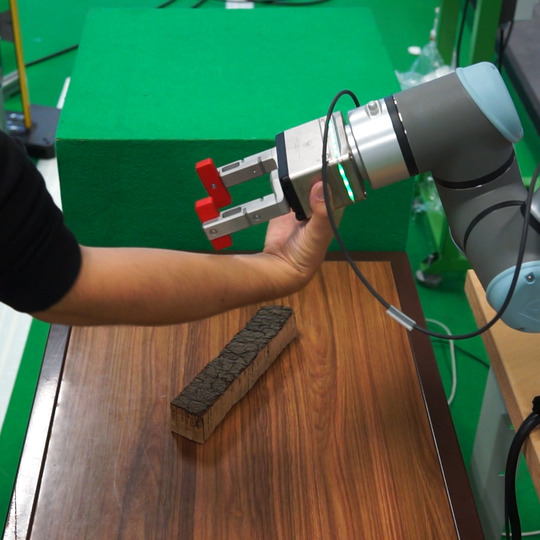
\includegraphics[width=.95\linewidth]{figs/chp6/hg_test_0.jpg}
    \end{subfigure}%
    \begin{subfigure}{.2\linewidth}
        \centering
        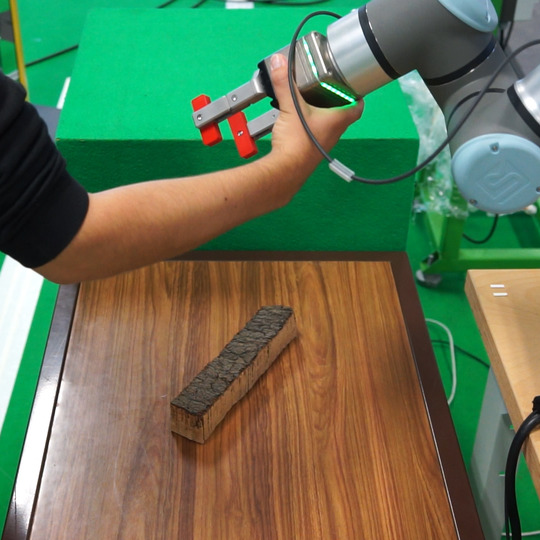
\includegraphics[width=.95\linewidth]{figs/chp6/hg_test_1.jpg}
    \end{subfigure}%
    \begin{subfigure}{.2\linewidth}
        \centering
        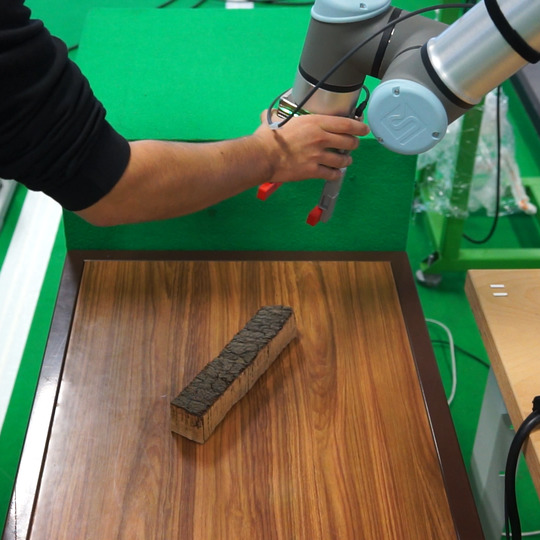
\includegraphics[width=.95\linewidth]{figs/chp6/hg_test_2.jpg}
    \end{subfigure}%
    \begin{subfigure}{.2\linewidth}
        \centering
        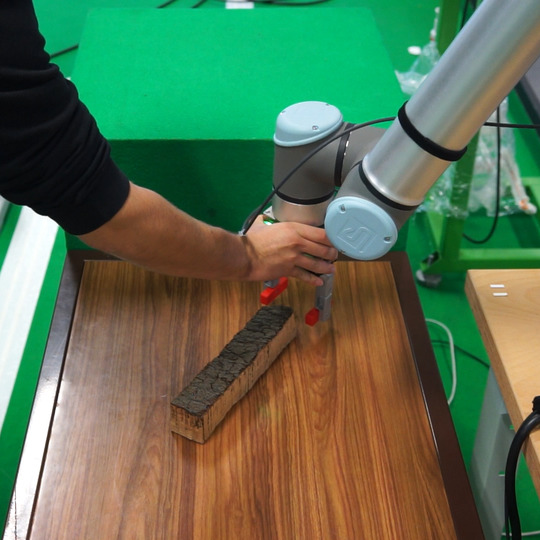
\includegraphics[width=.95\linewidth]{figs/chp6/hg_test_3.jpg}
    \end{subfigure}%
    \begin{subfigure}{.2\linewidth}
        \centering
        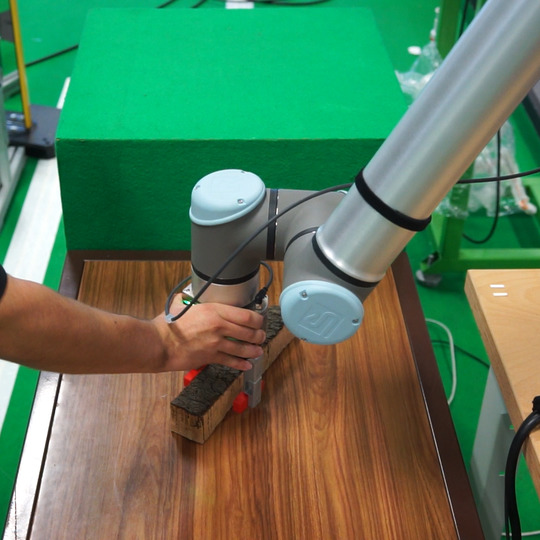
\includegraphics[width=.95\linewidth]{figs/chp6/hg_test_4.jpg}
    \end{subfigure}
    \caption{Succession of steps of the \ac{hg} test}
    \label{fig:hg_test}
\end{figure}

\par The test consists on  \ac{hg} the cobot with the objective of walking the gripper fingers through an object that is placed on the table. The system must compensate the \ac{ft} caused by the gripper in every orientation, therefore the cobot must only move due to external forces caused by the user. On the other hand, the user must align the gripper fingers with the object without difficulty. To test the system responsiveness, the user must walk the gripper through the object in a linear motion, while the gripper finger are aligned with it. THe succession of steps for this test is shown in \autoref{fig:hg_test}. 
The metrics for this test are effectiveness and responsiveness. Effective means that the user was able to complete the test, therefore the gripper weight was always correctly compensated and the robot only moved according to the force applied by the user. Responsive means that the robot motion was smooth and specifically in the part that the user must align the gripper fingers with the object on the table, while performing the linear movement, the griper fingers never touched the object. The results should be interpreted as number os successes in the amount of attempts. This test was performed 10 times in multiple settings of force thresholds from the compensation model, and the results are outlined in \autoref{tab:hand_guiding_test}. 


\begin{table}[h]
    \centering
    \begin{tabular}{|c|c|c|c|}
    \hline
    \textbf{\begin{tabular}[c]{@{}c@{}}Force\\ Threshold\end{tabular}} & \textbf{\begin{tabular}[c]{@{}c@{}}Test\\ Effectiveness\end{tabular}} & \textbf{\begin{tabular}[c]{@{}c@{}}Test\\ Responsiveness\end{tabular}} & \textbf{\begin{tabular}[c]{@{}c@{}}Qualitative\\ Performance\end{tabular}} \\ \hline
    \textbf{1N} & 3/10 & 10/10 & Unusable \\ \hline
    \textbf{2N} & 8/10 & 10/10 & Usable \\ \hline
    \textbf{3N} & 10/10 & 10/10 & Balanced \\ \hline
    \textbf{4N} & 10/10 & 9/10 & Satisfactory \\ \hline
    \textbf{5N} & 10/10 & 7/10 & Unresponsive \\ \hline
    \end{tabular}
    \caption{Results of the \ac{hg} performance test}
    \label{tab:hand_guiding_test}
\end{table}

\par A closer look at the results and an explanation of the qualitative performance will follow:
\begin{itemize}
    \item At 1N of force threshold, the system is unusable. The cobot is mostly moving by itself since the force threshold is too low. This result is expected and serves as a demonstration of the consequences of the inaccuracies of the \ac{ft} sensor.
    \item At 2N, the accuracy results are improved, but not entirely satisfactory. Due to physical interaction with the sensor, there were certain motions that would cause deviations on the \ac{ft} measurements. Despite this fact, with this setting the cobot is very responsive, reacting to very low amounts of force and allowing the gripper to be easily placed exactly where the user wants it to be.
    \item 3N proved to be the best threshold setting. It allowed the correct execution of every test and the loss on responsiveness was not perceptible. With the gripper attachment, 3N will be the default value for force threshold on the \ac{eef} weight compensation model.
    \item 4N and 5N allowed the same accuracy results obtained with 3N but at the cost of motion responsiveness. In short, the user would have to exert higher amounts of force on the \ac{eef} for it to move, causing degradation on its smoothness.
\end{itemize}

\par The general execution and behavior of the \ac{hg} task is a success. The goal of this test was not only to find the best system parameters to obtain the best possible behavior, but also to prove that the orchestration of \ac{ros} nodes and the algorithms they implement, proposed in this dissertation, is well founded and effective.

\subsection{Object Manipulation}

\par The object manipulation task requires the dynamic attachment of extra weight to the cobot \ac{eef}. It has been showed previously that the \ac{eef} weight compensation model supports dynamic changing of the weight and \ac{cog} parameters, but the performance of this manipulation task is directly proportional to the accurate measurement of this parameters.
\par The first test regarding this task should be to find both system and \ac{ft} sensor performance on correctly measuring the weight of the coupled object. In order to do this, a 1Kg iron weight will be gripped by the cobot 10 times in 6 different orientations. These orientations consist on vertically aligning each \ac{ft} axis, in each direction, with gravity, in order to obtain the accuracy of each measurement component, and can be seen in \autoref{fig:weight_poses}.

\begin{figure}[h]
    \centering
    \begin{subfigure}{.166\linewidth}
        \centering
        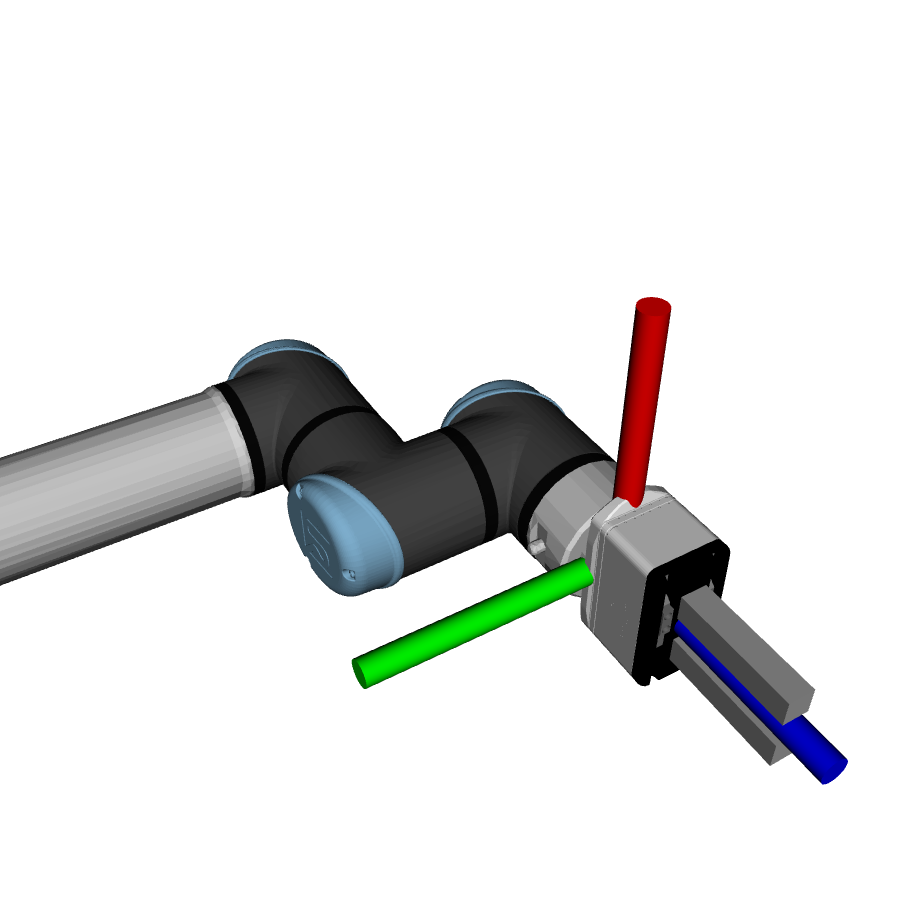
\includegraphics[width=\linewidth]{figs/chp6/weight_x_pos.png}
    \end{subfigure}%
    \begin{subfigure}{.166\linewidth}
        \centering
        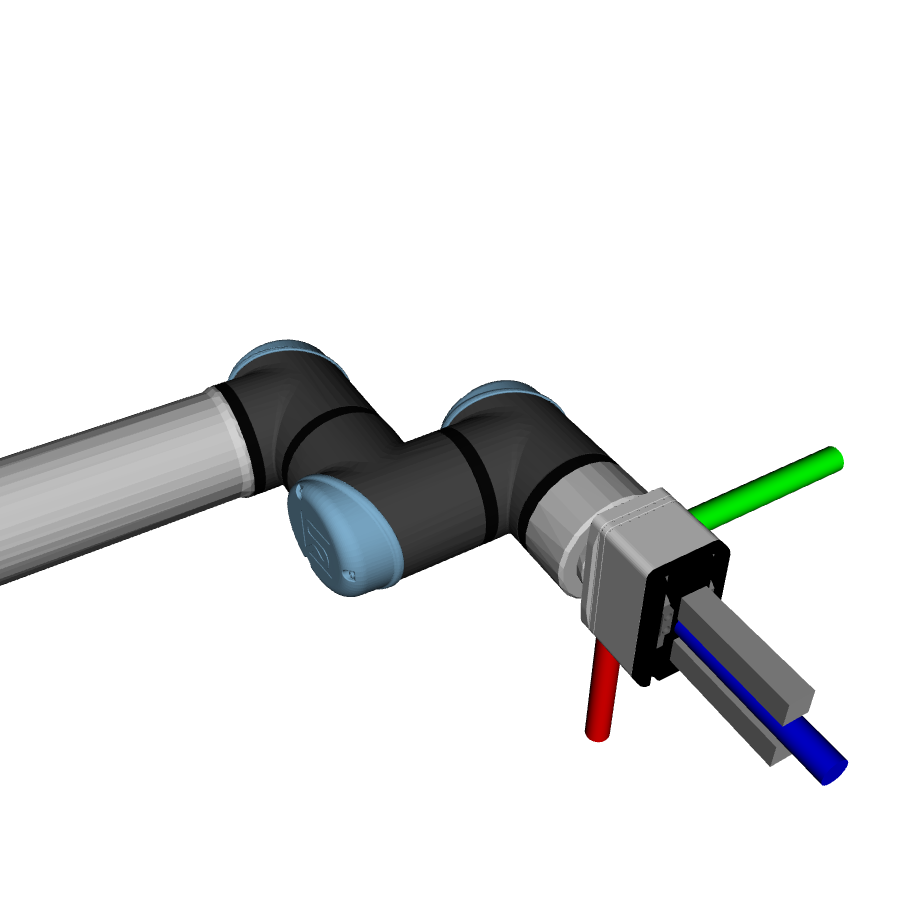
\includegraphics[width=\linewidth]{figs/chp6/weight_x_neg.png}
    \end{subfigure}%
    \begin{subfigure}{.166\linewidth}
        \centering
        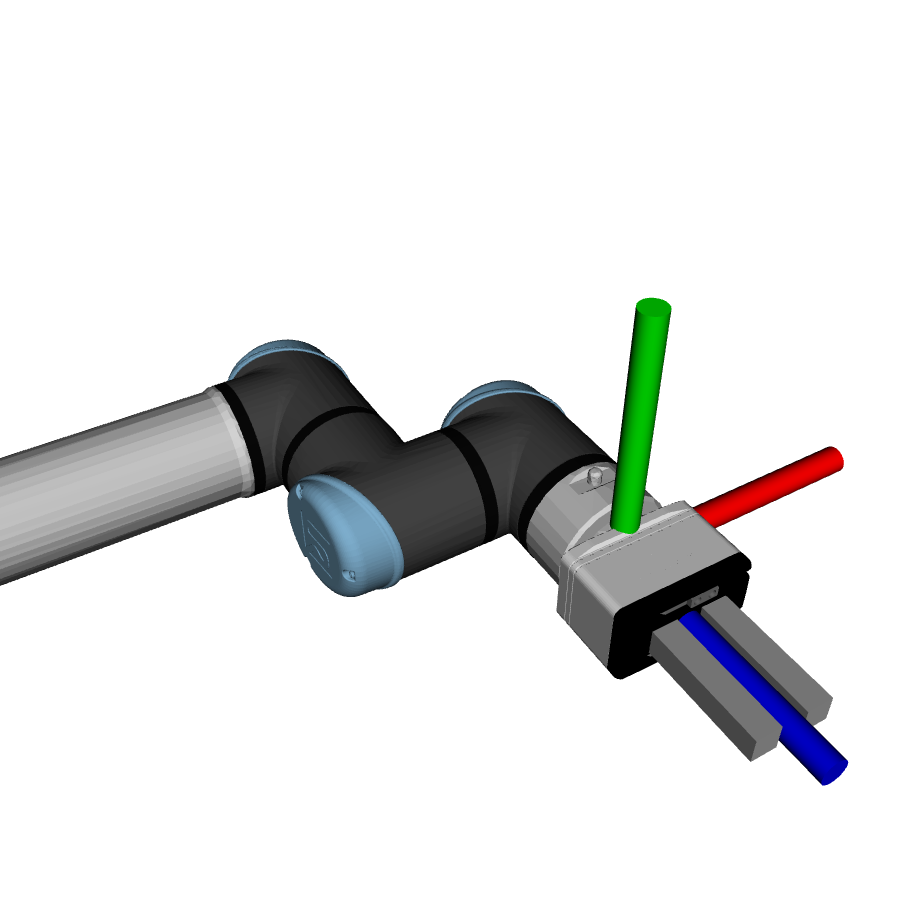
\includegraphics[width=\linewidth]{figs/chp6/weight_y_pos.png}
    \end{subfigure}%
    \begin{subfigure}{.166\linewidth}
        \centering
        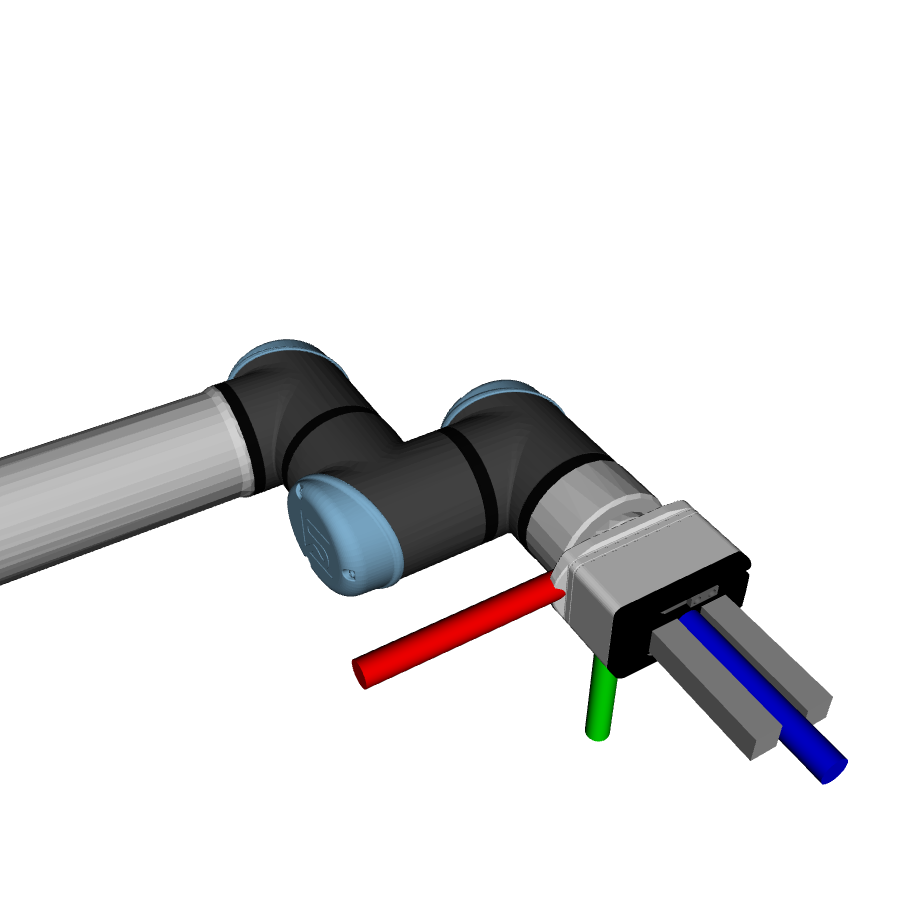
\includegraphics[width=\linewidth]{figs/chp6/weight_y_neg.png}
    \end{subfigure}%
    \begin{subfigure}{.166\linewidth}
        \centering
        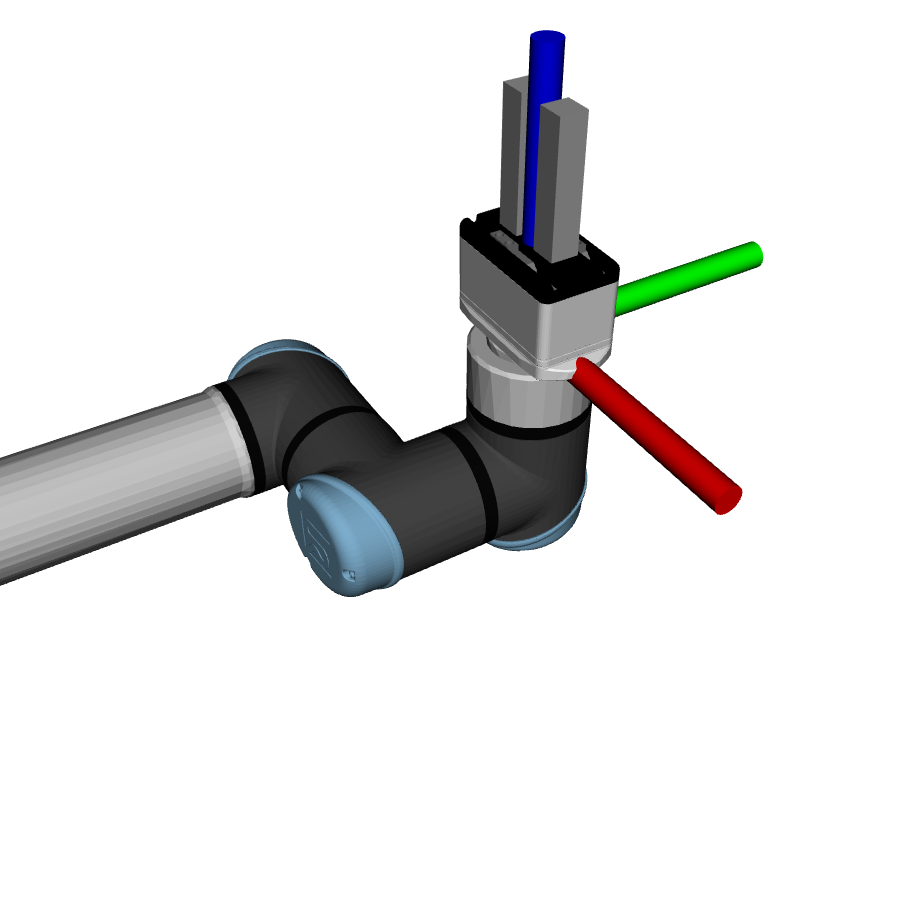
\includegraphics[width=\linewidth]{figs/chp6/weight_z_pos.png}
    \end{subfigure}%
    \begin{subfigure}{.166\linewidth}
        \centering
        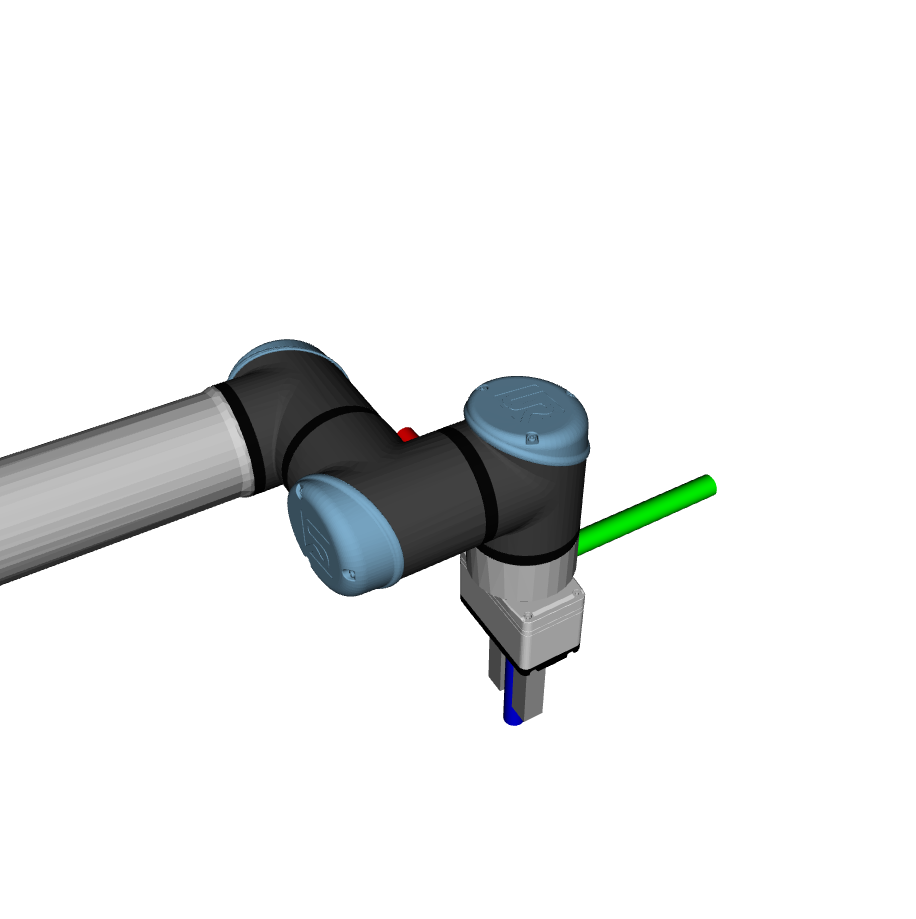
\includegraphics[width=\linewidth]{figs/chp6/weight_z_neg.png}
    \end{subfigure}
    \caption{6 different \ac{eef} weight measurement poses}
    \label{fig:weight_poses}
\end{figure}

\par The raw results are outlined in \autoref{fig:weight_result}. As it is evidently seen, changing the measuring axis has a significant effect on the reported measured weight.

\begin{figure}[h]
    \centering
    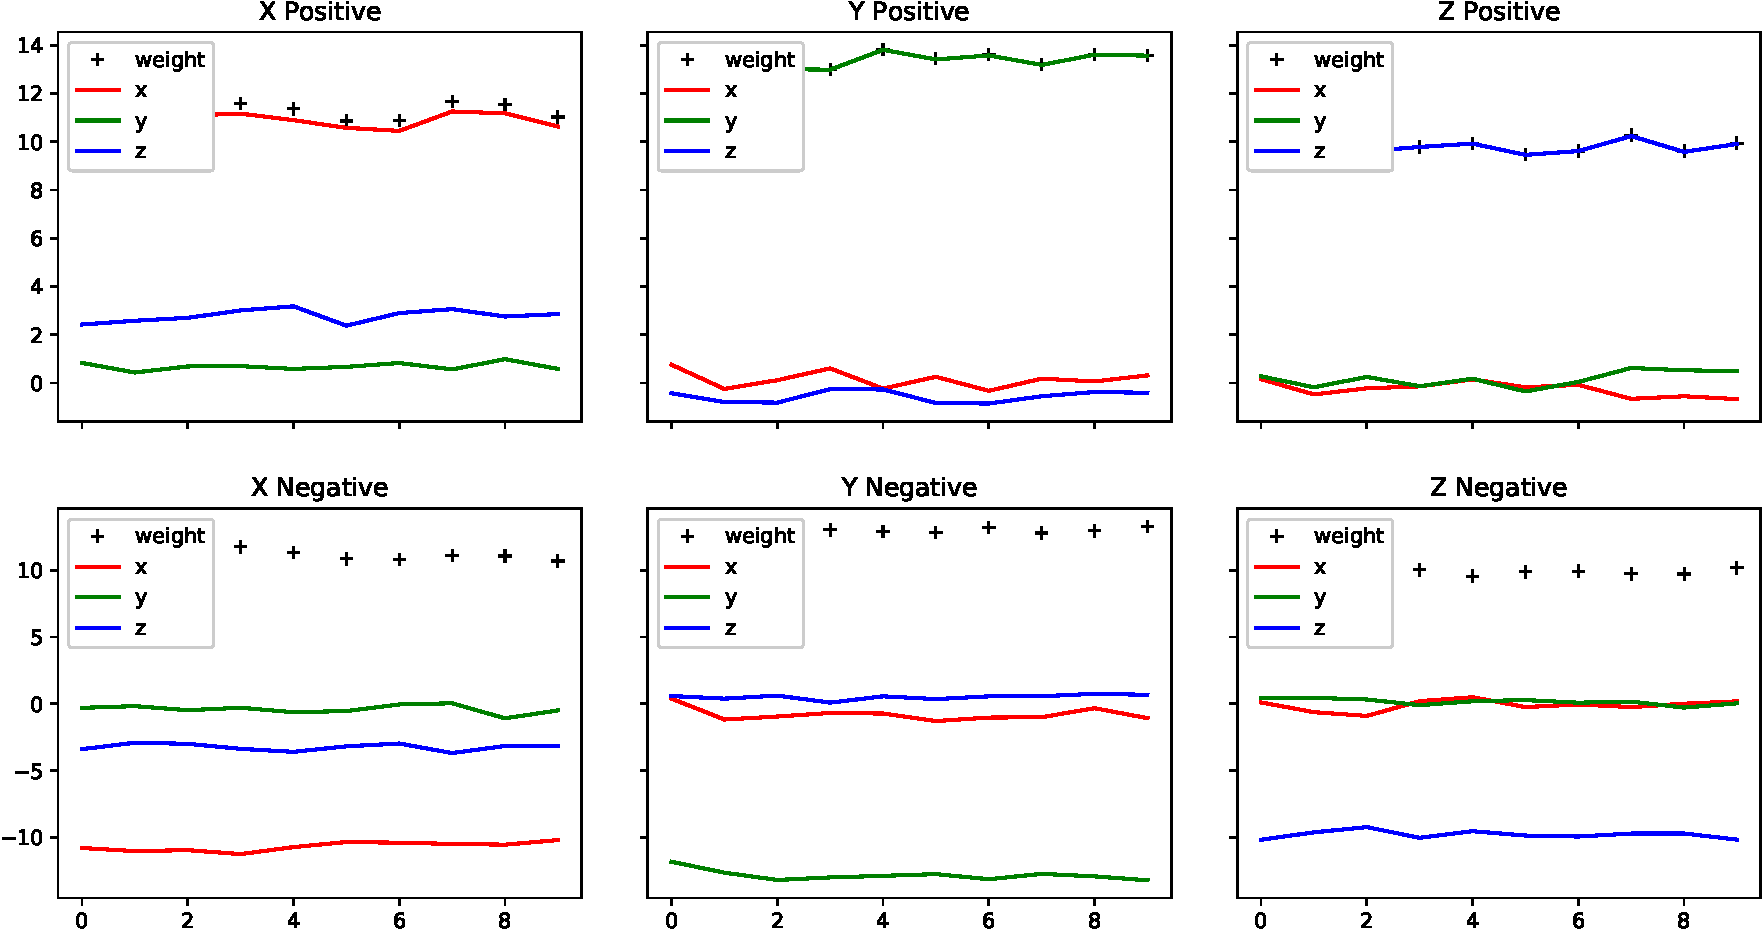
\includegraphics[width=0.8\linewidth]{figs/chp6/weight_measurements.pdf}
    \caption{Results of the weight measurement test in each position}
    \label{fig:weight_result}
\end{figure}

\par \autoref{tbl:weight_results} gives a closer look at the some statistics from the weight measurement tests. All values are to be read as weight in Kg.

\begin{table}[h]
    \centering
    \begin{tabular}{|l|c|c|c|}
    \hline
    \multicolumn{1}{|c|}{\textbf{\begin{tabular}[c]{@{}c@{}}Weight Test\end{tabular}}} & \textbf{Raw} & \textbf{\begin{tabular}[c]{@{}c@{}}\ac{dls}\\ Correction\end{tabular}} & \textbf{\begin{tabular}[c]{@{}c@{}}Scalar \\ Correction\end{tabular}} \\ \hline
    \textbf{X Positive} & 1.144 & 1.210 & 1.001 \\ \hline
    \textbf{X Negative} & 1.138 & 1.209 & 1.008 \\ \hline
    \textbf{Y Positive} & 1.369 & 1.229 & 1.025 \\ \hline
    \textbf{Y Negative} & 1.311 & 1.176 & 0.982 \\ \hline
    \textbf{Z Positive} & 0.992 & 1.219 & 1.016 \\ \hline
    \textbf{Z Negative} & 0.999 & 1.229 & 1.024 \\ \hline \hline
    \textbf{Average} & 1.159 & 1.213 & 1.011 \\ \hline
    \textbf{Std Dev} & 0.146 & 0.038 & 0.031 \\ \hline
    \end{tabular}
    \caption{Detailed results and statistics from the weight measurement tests}
    \label{tbl:weight_results}
\end{table}

\par At first, the raw values are neither precise nor accurate showing a wrong weight average and an arguably high standard deviation. Applying the correction constants obtained from \ac{dls} optimization in \autoref{ssec:ft_theory_model}, it is possible to improve the precision of the measurements, with a significantly lower standard deviation, but the final average weight value is still far from the correct. Applying a scalar correction with the value of 1.2 provides an accurate and precise weight measurement, with an improved and much lower standard deviation, meaning it is expected that in real use scenarios, the weight of a coupled object should only deviate, in the maximum, by this value.

\par Assuming the weight is correctly obtained, a real time test was performed to demonstrate that the \ac{eef} weight compensation model can sustain the same levels of accuracy independent of the weight coupled to the robot. \autoref{fig:object_result} shows a real time test where Wrist1 and Wrist2 joints are rotated causing multiple \ac{eef} orientations. Similar to previous real time tests the \ac{eef} weight is compensated with minimal error.

\begin{figure}[h]
    \centering
    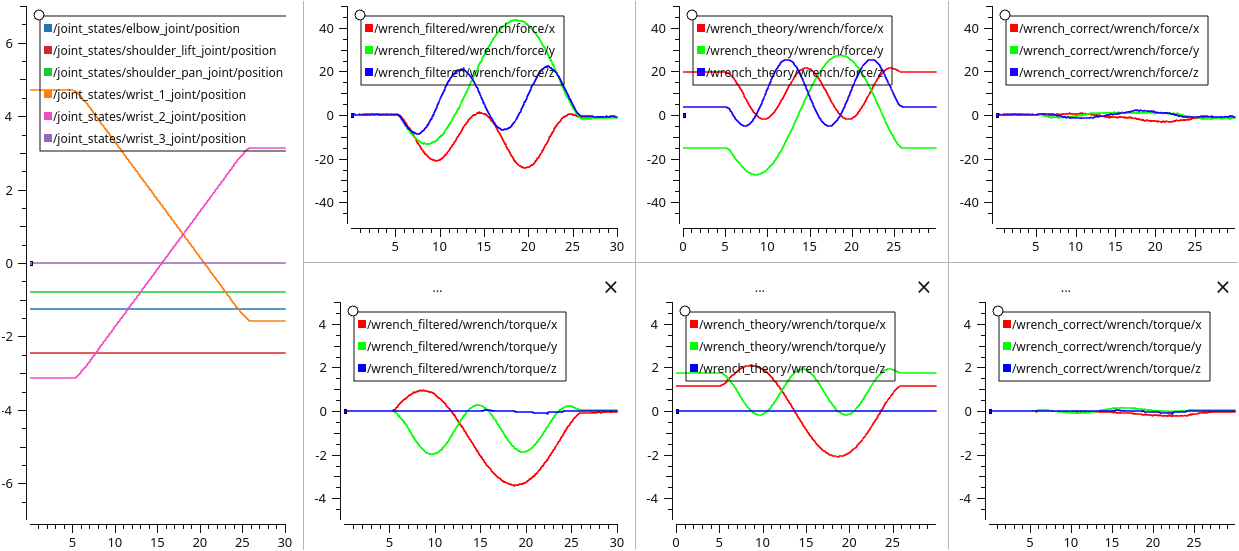
\includegraphics[width=0.9\linewidth]{figs/chp6/object_result.png}
    \caption{Result of the compensation architecture applied in a real time test}
    \label{fig:object_result}
\end{figure}

\begin{figure}[h]
    \centering
    \begin{subfigure}{.2\linewidth}
        \centering
        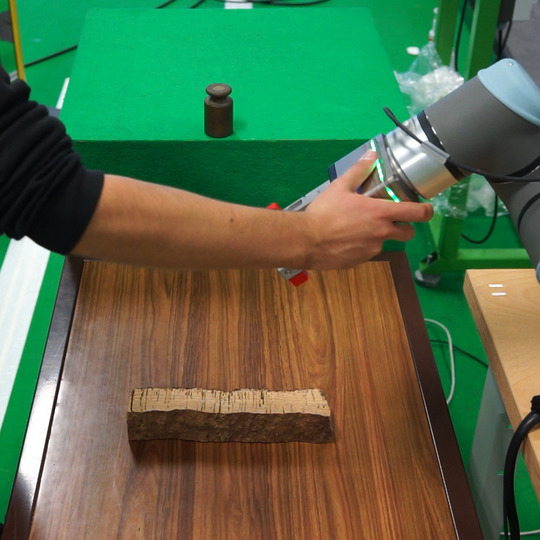
\includegraphics[width=.95\linewidth]{figs/chp6/om_test_0.jpg}
    \end{subfigure}%
    \begin{subfigure}{.2\linewidth}
        \centering
        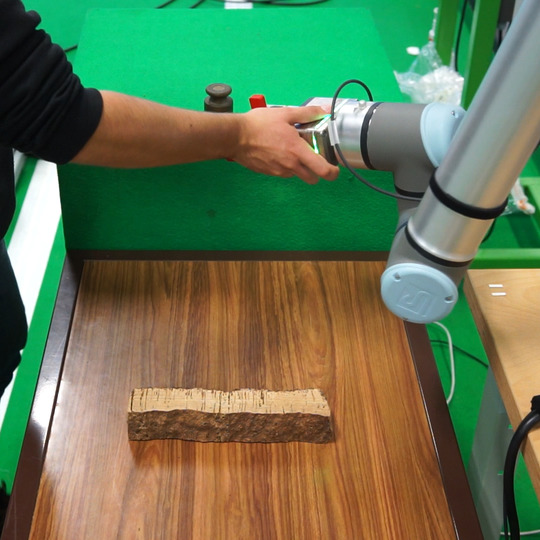
\includegraphics[width=.95\linewidth]{figs/chp6/om_test_1.jpg}
    \end{subfigure}%
    \begin{subfigure}{.2\linewidth}
        \centering
        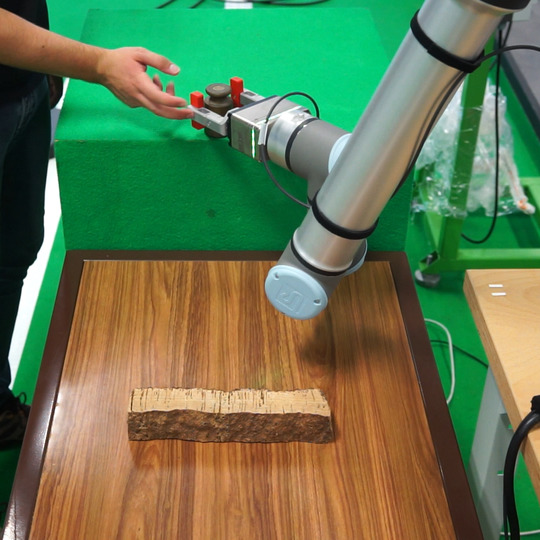
\includegraphics[width=.95\linewidth]{figs/chp6/om_test_2.jpg}
    \end{subfigure}%
    \begin{subfigure}{.2\linewidth}
        \centering
        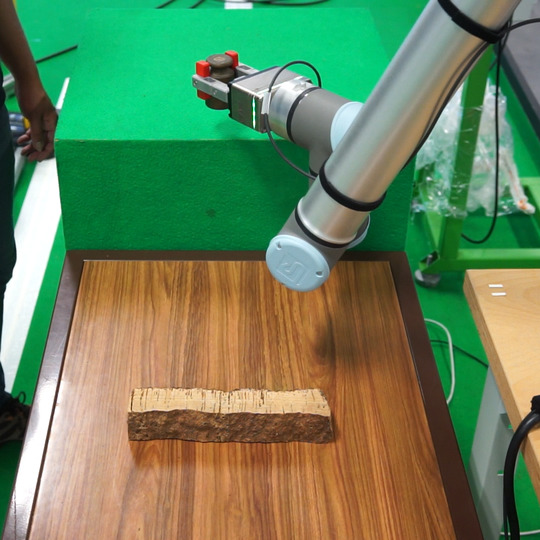
\includegraphics[width=.95\linewidth]{figs/chp6/om_test_3.jpg}
    \end{subfigure}%
    \begin{subfigure}{.2\linewidth}
        \centering
        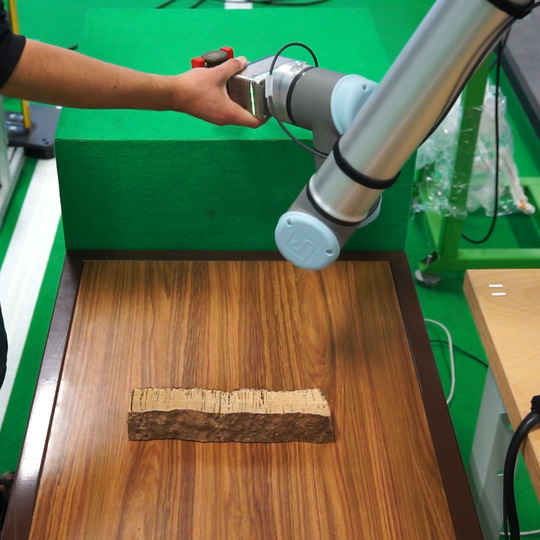
\includegraphics[width=.95\linewidth]{figs/chp6/om_test_4.jpg}
    \end{subfigure}
    \par\smallskip
    \begin{subfigure}{.2\linewidth}
        \centering
        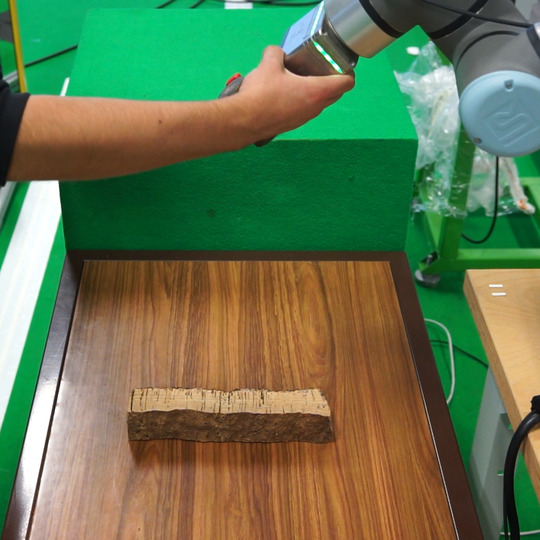
\includegraphics[width=.95\linewidth]{figs/chp6/om_test_5.jpg}
    \end{subfigure}%
    \begin{subfigure}{.2\linewidth}
        \centering
        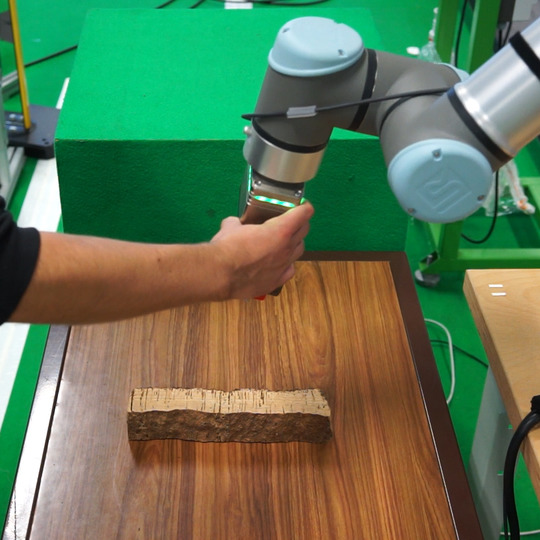
\includegraphics[width=.95\linewidth]{figs/chp6/om_test_6.jpg}
    \end{subfigure}%
    \begin{subfigure}{.2\linewidth}
        \centering
        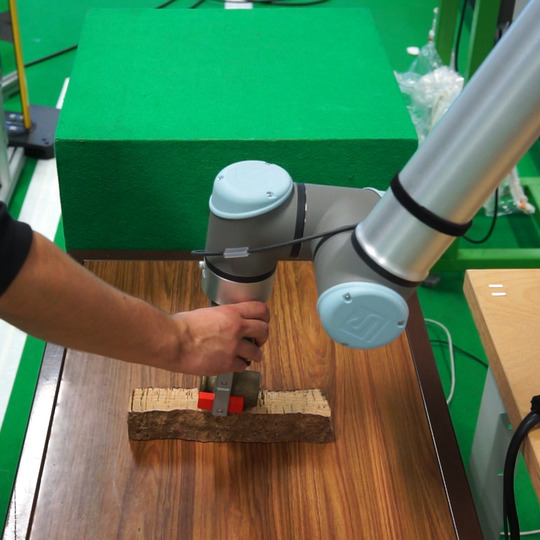
\includegraphics[width=.95\linewidth]{figs/chp6/om_test_7.jpg}
    \end{subfigure}%
    \begin{subfigure}{.2\linewidth}
        \centering
        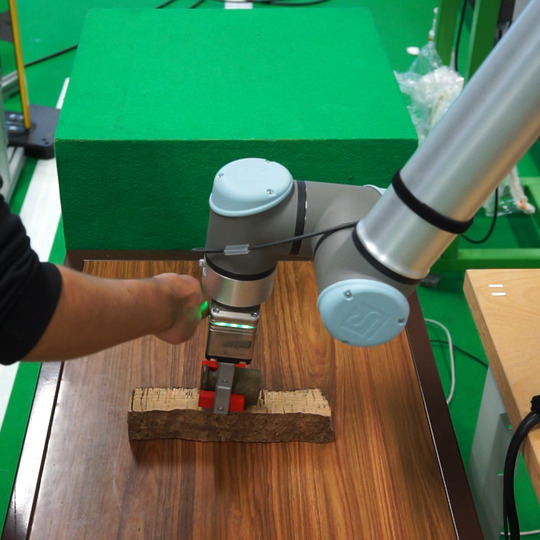
\includegraphics[width=.95\linewidth]{figs/chp6/om_test_8.jpg}
    \end{subfigure}%
    \begin{subfigure}{.2\linewidth}
        \centering
        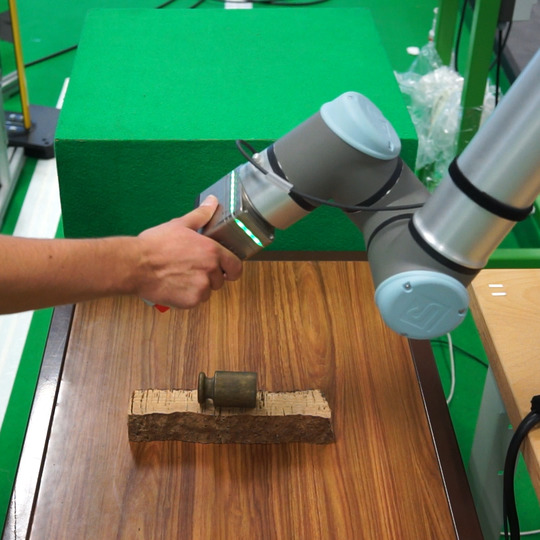
\includegraphics[width=.95\linewidth]{figs/chp6/om_test_9.jpg}
    \end{subfigure}
    \caption{Succession of steps of the object manipulation test}
    \label{fig:om_test}
\end{figure}

\par For the same reasons as in the \ac{hg} tests, weight compensation error is not enough to validate this task. Furthermore, since extra weight is added, it is suspected that the deviations caused by physical interaction with the \ac{ft} sensor will increase compared to the previous task. This time, the collaborative test consists on \ac{hg} the cobot, aligning it with a stationary object in the environment, give the order to grip it, wait for the system to calibrate its payload and manipulate the object with both linear and angular movements, in order to release it at another location in the environment. \autoref{fig:om_test} shows the succession of steps in this test. The evaluation metrics are the same as in th \ac{hg} test, and it was also repeated 10 times in each force threshold setting.

\begin{table}[h]
    \centering
    \begin{tabular}{|c|c|c|c|}
    \hline
    \textbf{\begin{tabular}[c]{@{}c@{}}Compensation\\ Accuracy\end{tabular}} & \textbf{\begin{tabular}[c]{@{}c@{}}Test\\ Effectiveness\end{tabular}} & \textbf{\begin{tabular}[c]{@{}c@{}}Test\\ Responsiveness\end{tabular}} & \textbf{\begin{tabular}[c]{@{}c@{}}Qualitative\\ Performance\end{tabular}} \\ \hline
    \textbf{1N} & 0/10 & 10/10 & Unusable \\ \hline
    \textbf{2N} & 3/10 & 10/10 & Unusable \\ \hline
    \textbf{3N} & 7/10 & 10/10 & Usable \\ \hline
    \textbf{4N} & 10/10 & 8/10 & Satisfactory \\ \hline
    \textbf{5N} & 10/10 & 5/10 & Unresponsive \\ \hline
    \end{tabular}
    \caption{Results of the object manipulation performance test}
    \label{tab:object_manipulation_test}
\end{table}

\par \autoref{tab:object_manipulation_test} presents the results of the test and similar to the previous task a qualitative interpretation of them will follow: 
\begin{itemize}
    \item Similar to the \ac{hg} task and for the same reasons, 1N of force threshold is unusable.
    \item At 2N, the results improve but there is still prone to a lot of deviations, therefore not enough.
    \item 3N show enough improvements on the results to be considered usable, since the majority of tests are completed. Given this fact, in a real manipulation scenario, the objective would be for the robot to never fail, even if it means sacrificing on responsiveness.
    \item 4N would be the ideal force threshold value for this task since it allows the completion of all the tests without significant sacrifice on motion responsiveness.
    \item 5N presents results similar to the \ac{hg} task where all tests are completed at the cost of motion smoothness.
\end{itemize}

\par In order for these tests to be successfully completed, the value of force threshold of the weight compensation model needed to be increased. This is caused by 2 factors: 

\begin{itemize}
    \item Increasing the \ac{eef} coupled weight increases the inaccuracies of the \ac{ft} sensor due to interaction with the user, as explained in \autoref{chapter:ft-sensor-correction}.
    \item The generation of force values from the theoretical \ac{ft} model is directly impacted by the configured value of object weight, which is measured and set in real time, when the robot grabs the object. Inaccuracies on weight measurement due to incorrect handover, or simply due to the arguably weak force accuracy specification value of 5.5N, can directly impact the performance of the theoretical model, whose ultimate goal is to model the behavior of the real \ac{ft} sensor.
\end{itemize}

\par The solution to this problem seems to rely on adapting the force threshold value of the theoretical \ac{ft} model according to the current payload weight. With a 1.5Kg gripper tool, 3N of force threshold meant manipulating the tool with a 1:5 force to motion ratio. Gripping a 1Kg iron weight, and increasing the force threshold to 5N allows to maintain the same ratio and be able to successfully and accurately manipulate the conjoint weight. The loss on responsiveness is an acceptable tradeoff for the fact that, in the end, the tests in question were effectively completed. 

\subsection{Collision Avoidance}
\label{sec:colision_tests}

\par Make a XYZ graph with the predefined trajectory and the collision avoidance trajectory
\par Make a table with varying number of objects and benchmark completeness
\par Make a table with the response times of the object detection (gazebo)

\section{System Stability}

\par A more general performance metric is the ability for the system to maintain activity for long periods of time. There are several factors that prevent this from happen. During the execution of the previous tests and any other time directly interfacing with the robot, there were some events that injured the overall experience.
\par For instance, at random instances, when the robot had been correctly functioning for a certain amount of time, e.g. 20 minutes, the system will lose connection with the robot. More specifically, the \ac{ur} \ac{ros} driver looses connection to the \ac{rtde} interface, or in some instances, the client program that is running on the robot, requesting commands to the driver suddenly stops its execution. The cause of this problem was not studied since there was no observable pattern on the instances that is happened. The solution was to call the \textbackslash\textit{resend\_robot\_program} \ac{ros} service made available by the driver and the connection would resume.
\par Another example is the fact that, because we are dealing with a cobot and the joints are force sensitive, when applying large amounts of force on the \ac{eef}, the cobot will make a protective stop, giving the user a violation alert, explaining that a force or speed limit was exceeded. Other examples of protective stops are prone to happen when the user couples high amounts of weight to the \ac{eef}. This happens because this weight is not reported to the \ac{ur10e} Polyscope interface. It is obvious that the \ac{ur10e} internal controllers need to know the correct value of payload in order to correctly calculate the necessary torques to apply in each joint, but as was explained in \autoref{ssec:ft_internal_comp}, not reporting the payload parameters to the \ac{ur10e} internal system is a necessary tradeoff for obtaining cohesive \ac{ft} measurements on the \ac{eef}.
\par A final remark on system performance gives light to the fact that all components of this system were tested and implemented on a laptop with an Intel Core i7-8550U and 16Gb of \acs{ram}. 